\section{Introduction}
Within the first batch of the ClimAmazon project 20 samples have been processed so far in total. 
From these in total 20 samples are 16 samples from the boat cruises in June and November 2013, two reference materials (Til-1 and San Joaquin Soil) and two blanks \ref{tab:CA_samples}.

\begin{table}[h]
\centering
\caption{ClimAmazon processed samples of the first batch}
\label{tab:CA_samples}
\begin{tabular}{|l|l|l|l|l|l|l|l|}
\hline
labName & Site No.             & Depth & Sampling site          & River   & Longitude    & Latitude     & Sampling date \\ \hline
CA-1    & CA-0613-2 8m         & 8     & Alter do Chão          & Tapajós & -55.00468    & -2.4745      & 19.06.13      \\ \hline
CA-2    & CA-0613-2  17m       & 17    & Alter do Chão          & Tapajós & -55.00468    & -2.4745      & 19.06.13      \\ \hline
CA-3    & CA-0613-3 P1 surface & 0     & Óbidos                 & Amazon  & -55.493433   & -1.940758    & 21.06.13      \\ \hline
CA-4    & CA-0613-3 P1 15m     & 15    & Óbidos                 & Amazon  & -55.493433   & -1.940758    & 21.06.13      \\ \hline
CA-5    & CA-0613-3 P1 45m     & 45    & Óbidos                 & Amazon  & -55.493433   & -1.940758    & 21.06.13      \\ \hline
CA-6    & CA-0613-6b surface   & 0     & Almeirim               & Amazon  & -52.605166   & -1.576361    & 21.06.13      \\ \hline
CA-7    & CA-0613-7b surface   & 0     & Porto de Moz           & Xingu   & -52.15692778 & -1.627480556 & 21.06.13      \\ \hline
CA-8    & CA-0613-10  surface  & 0     & Macapa North Profile 2 & Amazon  & -51.05756    & -0.056803    & 21.06.13      \\ \hline
CA-9    & CA-0613-10  10m      & 10    & Macapa North Profile 2 & Amazon  & -51.05756    & -0.056803    & 21.06.13      \\ \hline
CA-10   & CA-0613-10  25m      & 25    & Macapa North Profile 2 & Amazon  & -51.05756    & -0.056803    & 21.06.13      \\ \hline
CA-11   & CA-1113-1a           & 0     & Obidos                 & Amazon  & -55.49869    & -1.93993     & 31.10.2013    \\ \hline
CA-12   & CA-1113-1a           & 20    & Obidos                 & Amazon  & -55.49869    & -1.93993     & 31.10.2013    \\ \hline
CA-13   & CA-1113-1a           & 40    & Obidos                 & Amazon  & -55.49869    & -1.93993     & 31.10.2013    \\ \hline
CA-14   & CA-1113-9            & 0     & Macapa Profile         & Amazon  & -51.51281    & -0.5449      & 12.11.2013    \\ \hline
CA-15   & CA-1113-9            & 12    & Macapa Profile         & Amazon  & -51.51281    & -0.5449      & 12.11.2013    \\ \hline
CA-16   & CA-1113-9            & 22    & Macapa Profile         & Amazon  & -51.51281    & -0.5449      & 12.11.2013    \\ \hline
CA-17   & Til-1                &       & soil standard          &         &              &              &               \\ \hline
CA-18   & 2709a-SJS            &       & soil standard          &         &              &              &               \\ \hline
CA-19   & blank1               &       &                        &         &              &              &               \\ \hline
CA-20   & blank2               &       &                        &         &              &              &               \\ \hline
\end{tabular}
\end{table}

\begin{figure}[htbp]
	\centering
	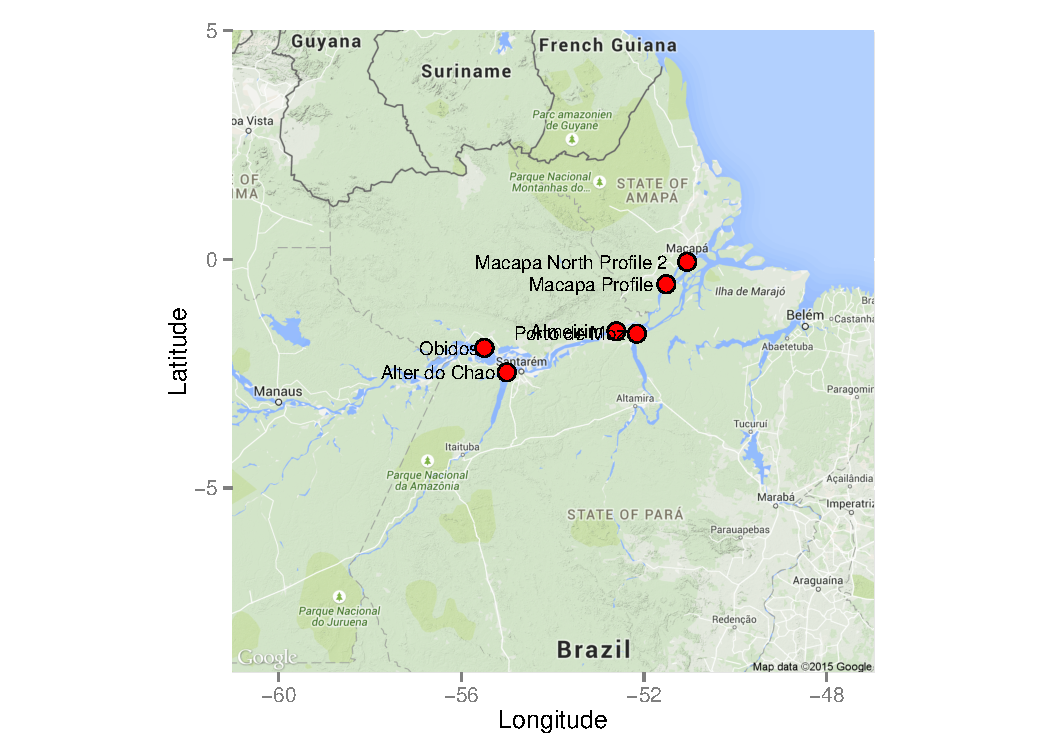
\includegraphics[width=0.95\textwidth]{figures/climAmazoneMap.pdf}
	\caption{Red dots show the sampling points of the first ClimAmazon batch processed.}
	\label{fig:climAmazonSampleMap}
\end{figure}